%\chapter*{Неделя 3}
\protect\thispagestyle{fancy}
\section{}
Гармонический сигнал $x(t) = \cos(2 \pi f_0 t)$, $f_0 = 35$ Гц, дискретизован с частотой дискретизации $f_d = 140$ Гц. Найти и изобразить по модулю ДПФ и ДВПФ отрезка сигнала из восьми отсчётов.

\begin{align*}
	&x(t) =  \cos(2 \pi f_0 t) = \dfrac{1}{2}e^{j2\pi f_0 t} + \dfrac{1}{2}e^{-j2\pi f_0 t},\\
	&\Capit{X}(\nu) = \dfrac{1}{2}\sum\limits_{m = -\infty}^{+\infty}\Big[\delta(\nu - \nu_0 -m) + \delta(\nu + \nu_0 - m)\Big],\ \text{где}\ \nu_0 = \dfrac{f_0}{f_d} = \dfrac{35}{140} = \dfrac{1}{4}.\\
	&\Capit{X}_{8}(\nu) = \Capit{X}(\nu) \otimes \Capit{D}_{8}(\nu)\footnotemark  = \dfrac{1}{2} \Big[\Capit{D}_{8}(\nu - \nu_0) + \Capit{D}_{8}(\nu + \nu_0) \Big]
	= \dfrac{1}{2} \Big[e^{-j7\pi (\nu - \nu_0)}\dfrac{\sin(8\pi(\nu - \nu_0))}{\sin(\pi(\nu - \nu_0))} + e^{-j7\pi (\nu + \nu_0)}\dfrac{\sin(8\pi(\nu + \nu_0))}{\sin(\pi(\nu + \nu_0))} \Big].\\
	&\Capit{X}_{8}[n] = \sum\limits_{k=0}^{7} \cos(2 \pi \nu_0 k) e^{-j 2\pi \frac{n}{8}k} = 
	\dfrac{1}{2} \sum\limits_{k=0}^{7} \Big[e^{j 2\pi k (2 - n)/8} + e^{-j 2\pi k (2 + n)/8} \Big] =
	\begin{cases}
		4,\quad \text{если} \ n\%8 \in \{2, 6\},\\
		0,\quad \text{если} \ n\%8 \not\in \{2, 6\}.
	\end{cases}
\end{align*}
\footnotetext{$\Capit{D}_8(\nu)$ -- ДВПФ прямоугольного окна длительностью $8$.}

\begin{figure}[!h]
	\centering
	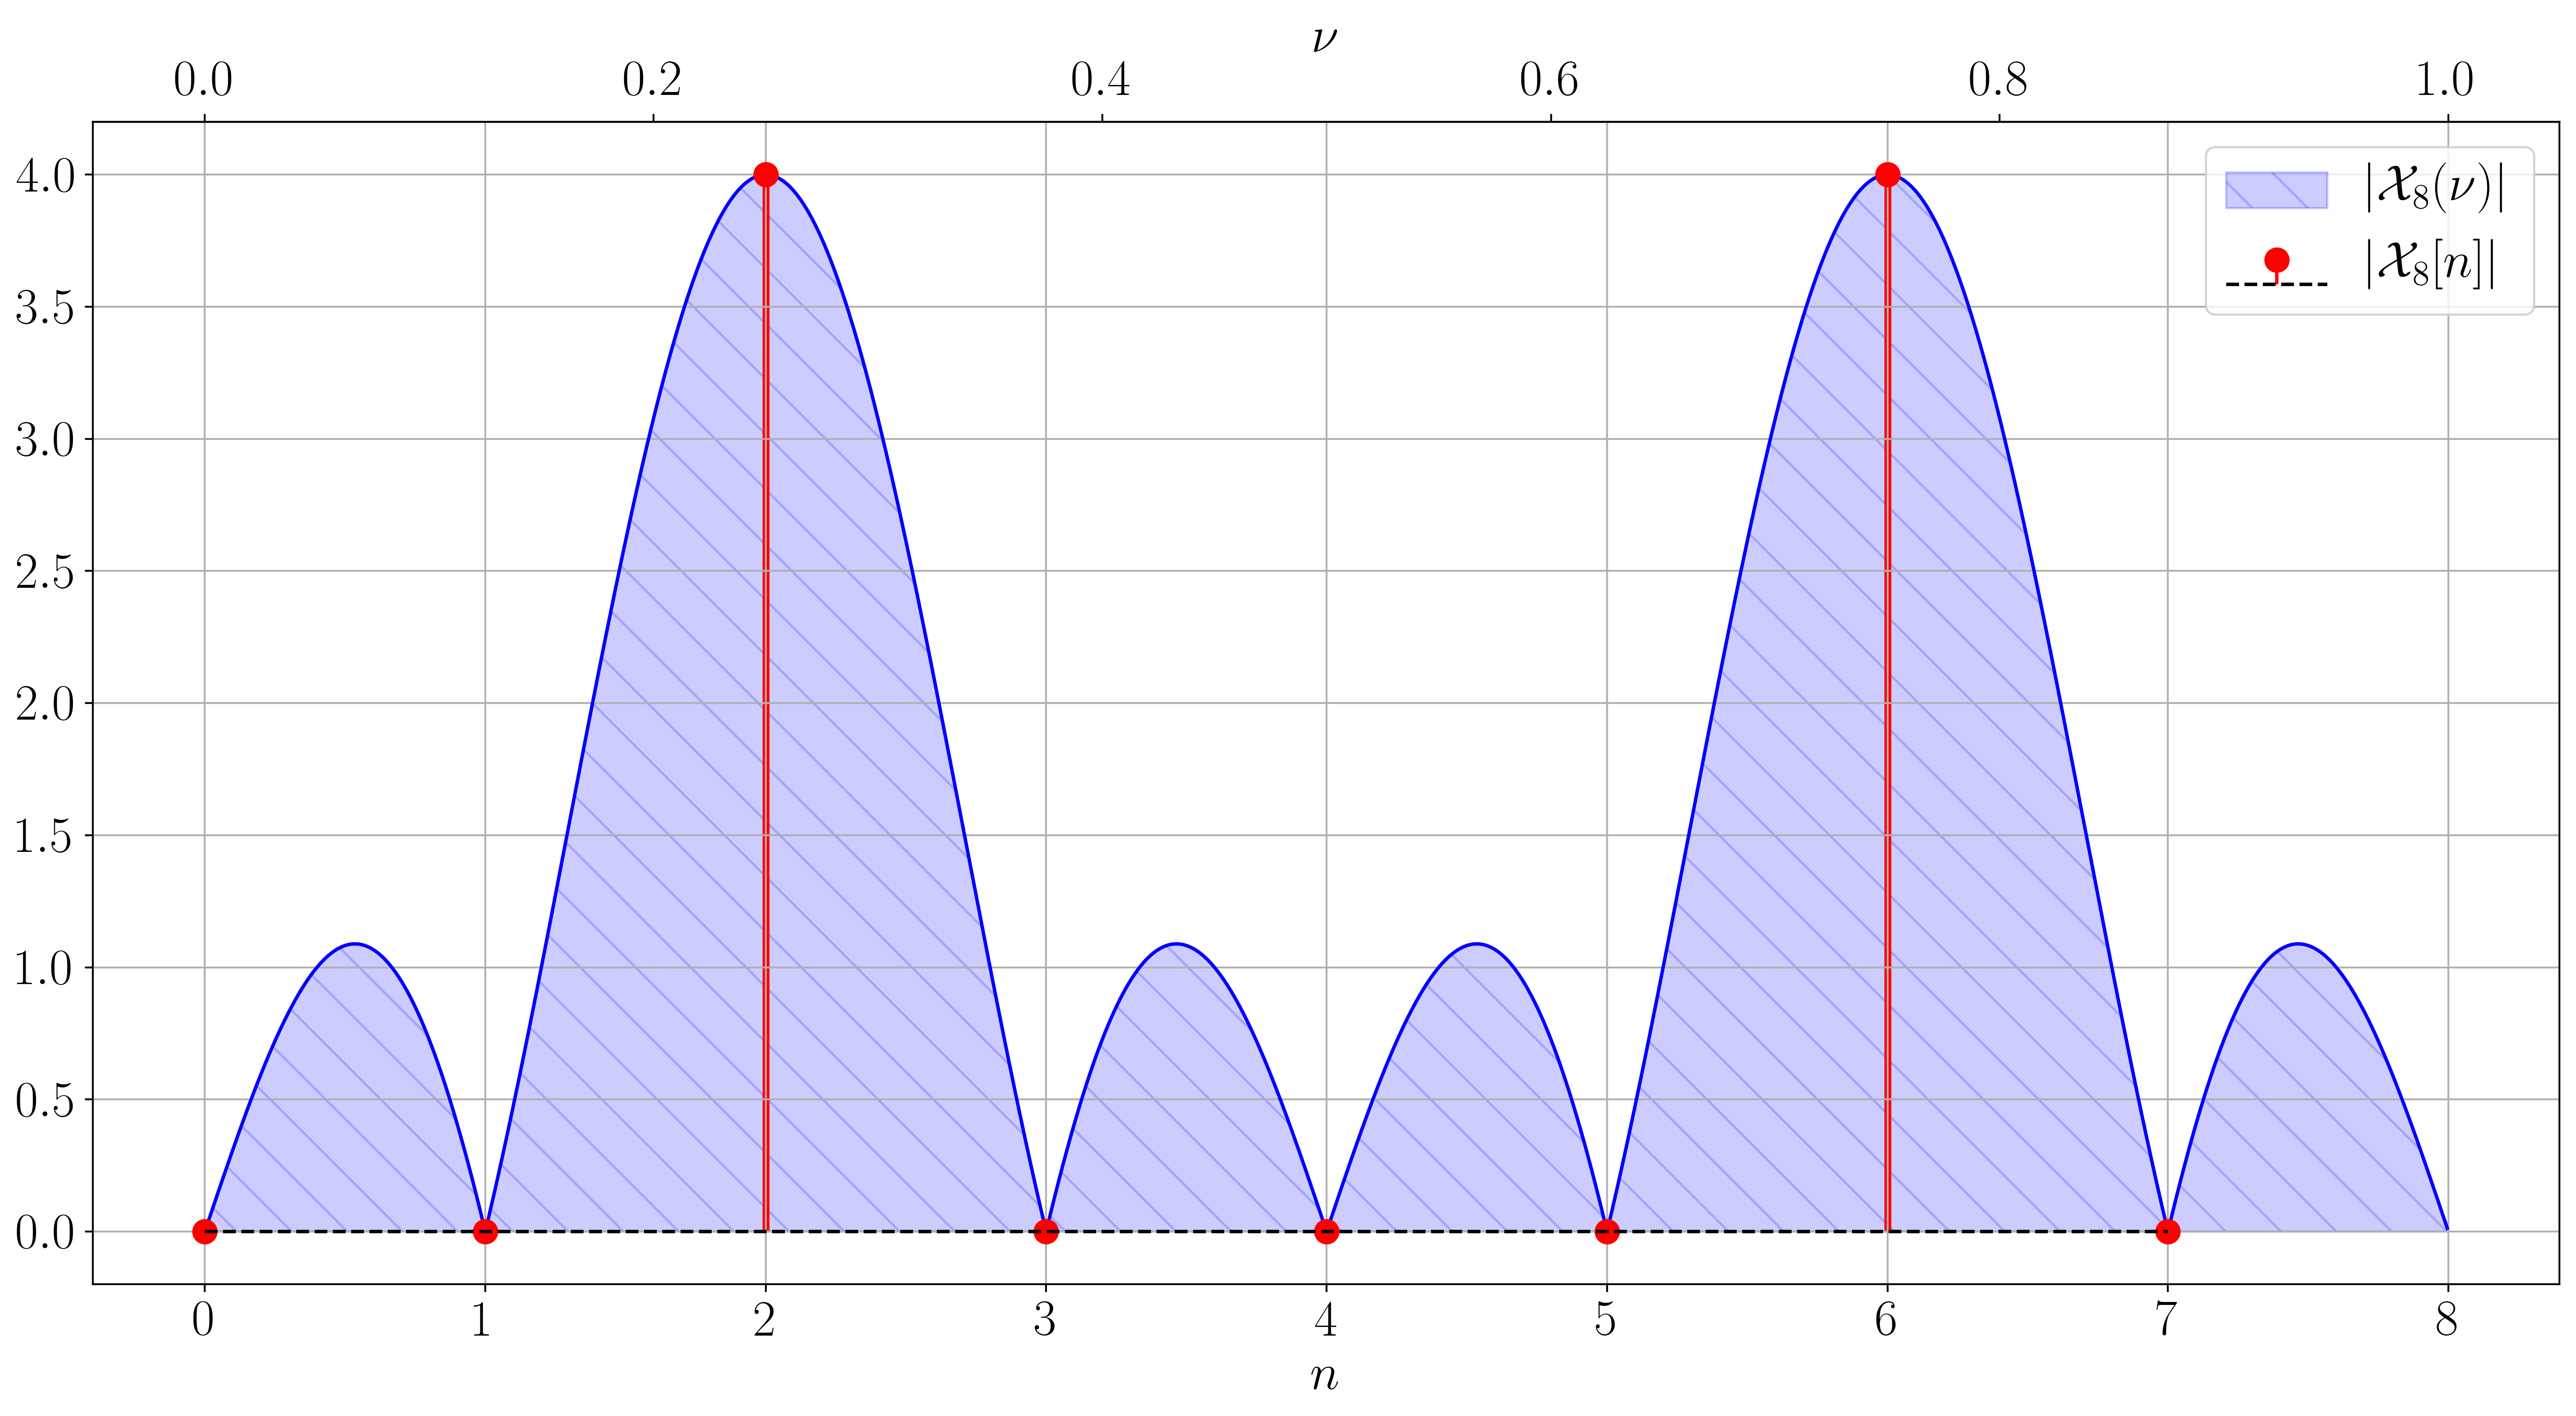
\includegraphics[width=1.0\columnwidth]{pics/fall/3/3-1.png}
	\label{fig:3-1}
\end{figure}

\newpage
\section{}

\begin{figure}[!h]
	\centering
	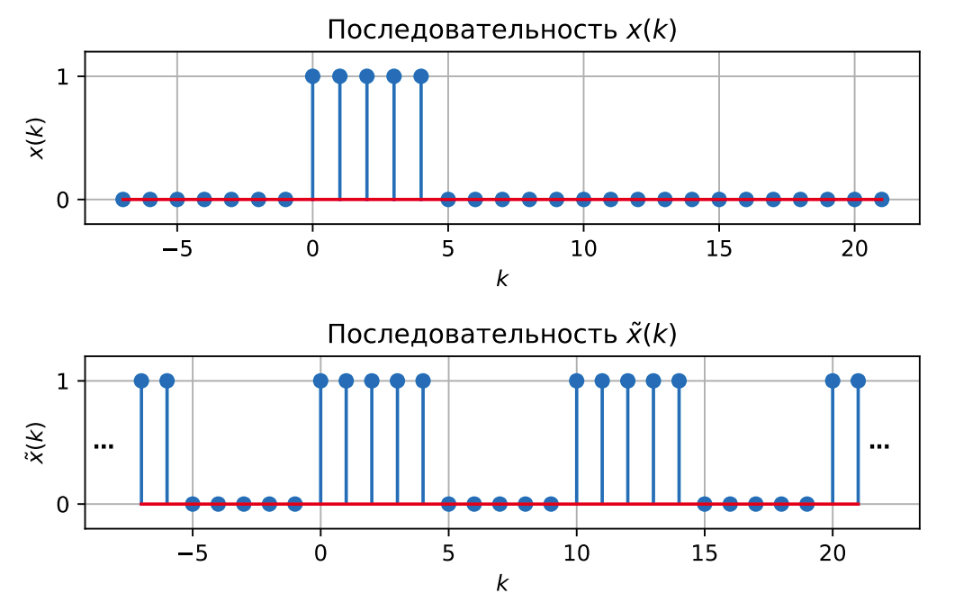
\includegraphics[width=0.5\columnwidth]{pics/fall/3/3-2-0.png}
	\label{fig:3-2-0}
\end{figure}


Изобразить модули коэффициентов ДПФ $5$-точечной последовательности $x[k]$ (пятиточечного) и её периодического продолжения $\widetilde{x}[k]$ с периодом $10$.




\begin{align*}
	&\Capit{X}[n] = \sum \limits_{k=0}^{4} x[k] e^{-j 2\pi \frac{n}{5}k} = \sum \limits_{k=0}^{5} e^{-j 2\pi \frac{n}{5}k} = \dfrac{1 - e^{-j 2\pi n}}{1 - e^{-j 2\pi \frac{n}{5}}} = 
	\dfrac{e^{-j \pi n}}{e^{-j \pi \frac{n}{5}}} \dfrac{\sin(\pi n)}{\sin\big(\frac{\pi n}{5}\big)} = 
	\begin{cases}
		5,\quad \text{если} \ n\%5 = 0,\\
		0,\quad \text{если} \ n\%5 \neq 0.
	\end{cases}\\
	&\widetilde{\Capit{X}}[n]  = \sum \limits_{k=0}^{9} x[k] e^{-j 2\pi \frac{n}{10}k} = 
	\sum \limits_{k=0}^{4} e^{-j 2\pi \frac{n}{10}k} = \dfrac{1 - e^{-j 2\pi \frac{n}{2}}}{1 - e^{-j 2\pi \frac{n}{10}}} = 
	\dfrac{e^{-j \pi \frac{n}{2}}}{e^{-j \pi \frac{n}{10}}} \dfrac{\sin\big(\frac{\pi n}{2}\big)}{\sin\big(\frac{\pi n}{5}\big)}.
\end{align*}

\begin{figure}[!h]
	\centering
	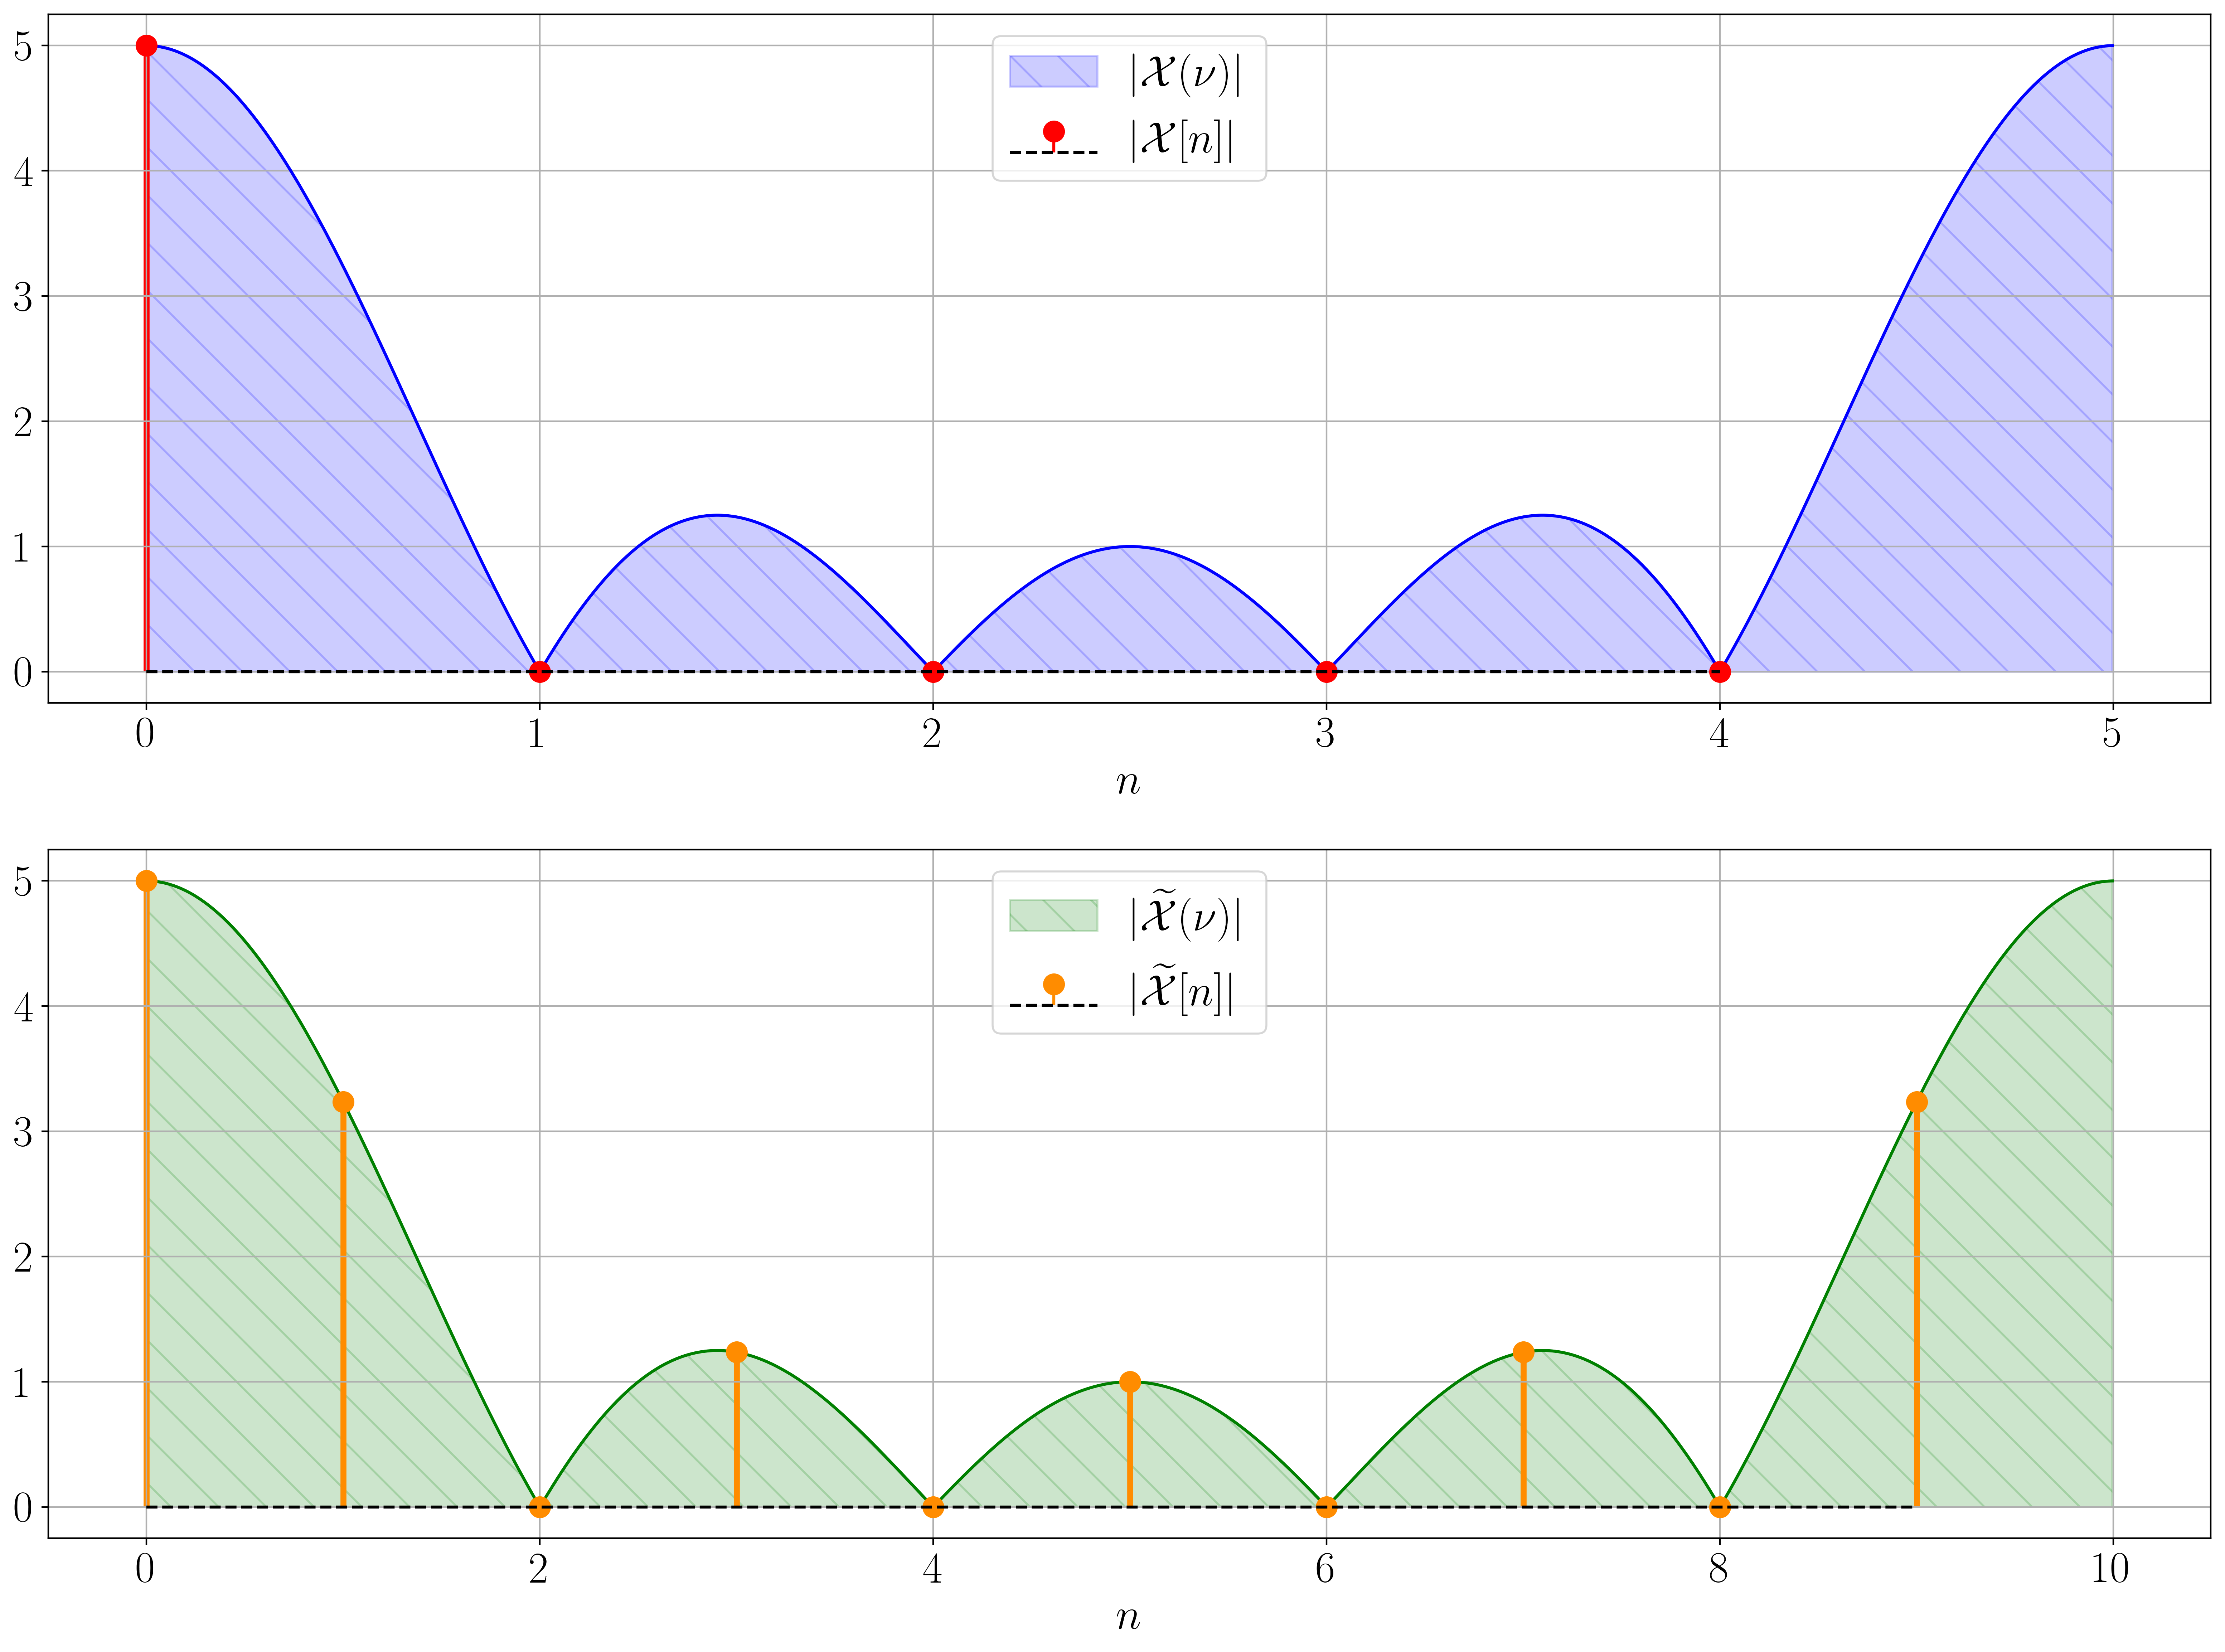
\includegraphics[width=0.9\columnwidth]{pics/fall/3/3-2.png}
	\label{fig:3-2}
\end{figure}


\section{}
Пусть $\Capit{X}[n]$ -- четырёхточечное ДПФ последовательности $x[k]$, изображённой на графике.

\begin{figure}[!h]
	\centering
	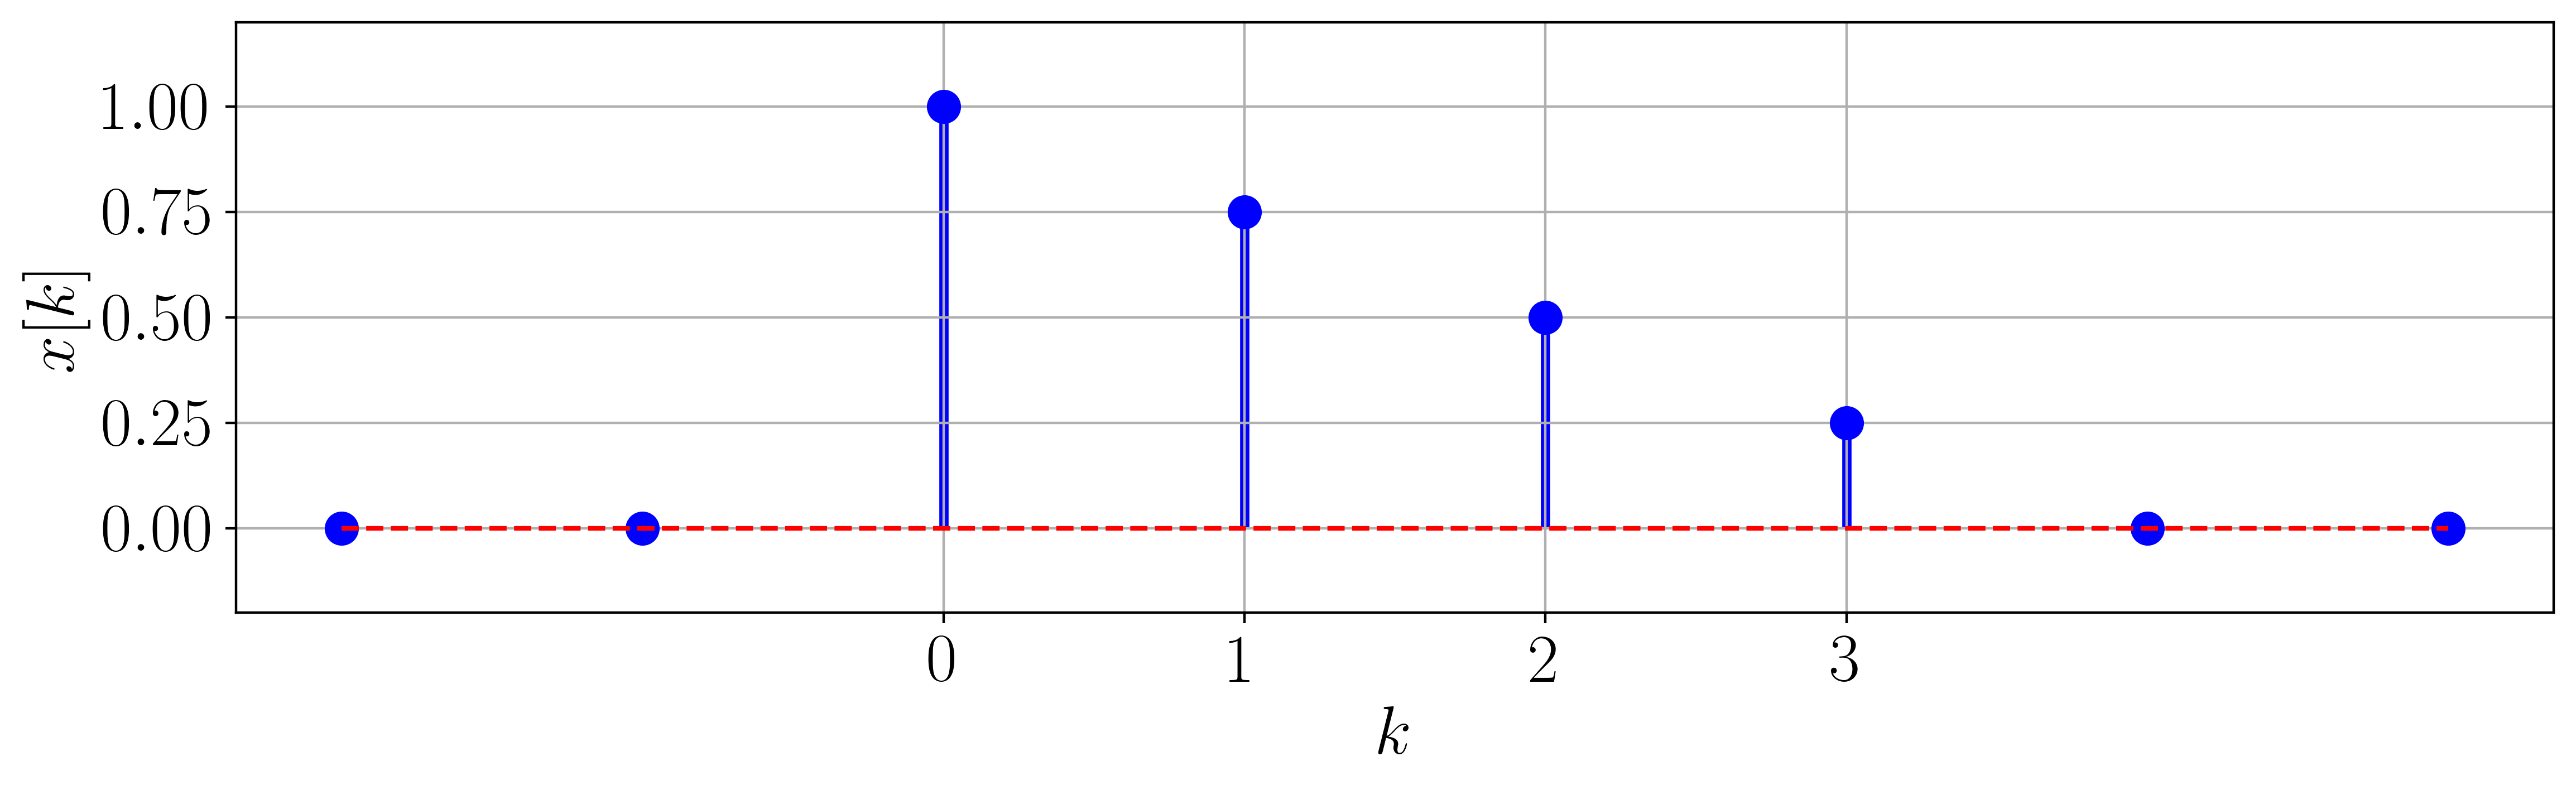
\includegraphics[width=0.8\columnwidth]{pics/fall/3/3-3-1.png}
	\label{fig:3-3-1}
\end{figure}

Изобразить последовательность $y[k]$, ДПФ которой имеет вид $\Capit{Y}[n] = \exp\Big(-j \dfrac{2\pi}{4}n\Big)\Capit{X}[n]$.

По теореме запаздывания имеем:
\begin{equation*}
	\Capit{Y}[n] = \exp\Big(-j \dfrac{2\pi}{4}n\Big)\Capit{X}[n]\ \xlongleftrightarrow{DFT}\ x[k-1]_{4} = y[k].
\end{equation*}

То есть последовательность $y[k]$ получается путём циклического сдвига $x[k]$ на $1$ отсчёт вправо.
\begin{figure}[!h]
	\centering
	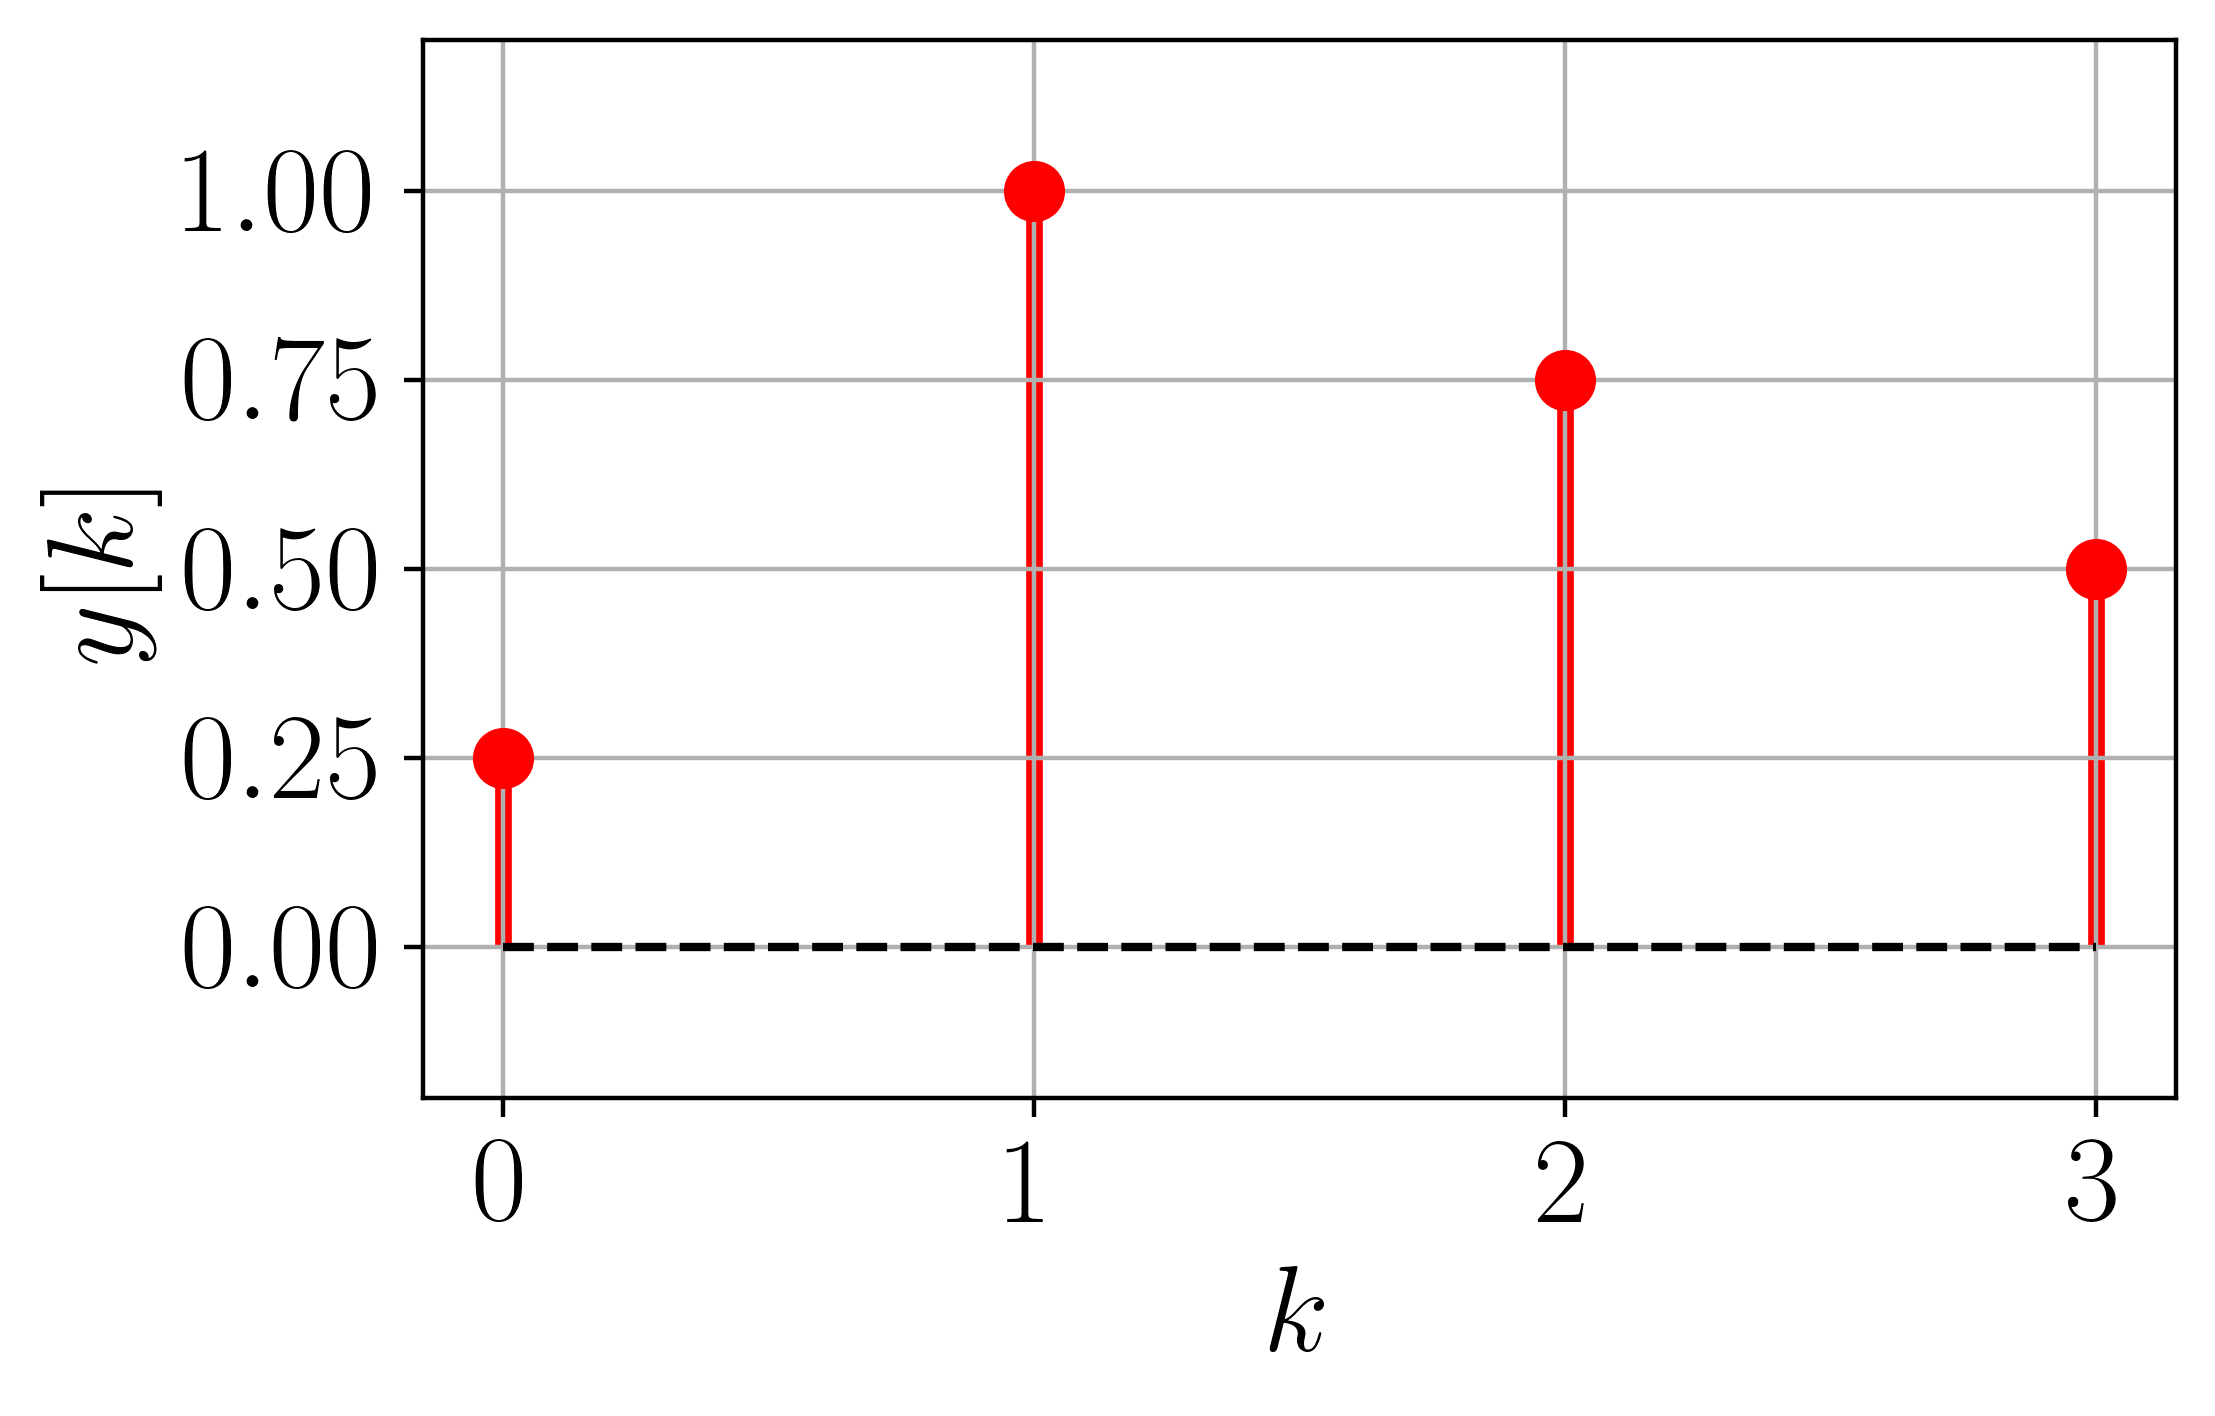
\includegraphics[width=0.4\columnwidth]{pics/fall/3/3-3-2.png}
	\label{fig:3-3-2}
\end{figure}
